\documentclass[10pt]{article}
\usepackage{latexsym}
\usepackage{natbib}
\usepackage{graphicx}
\usepackage{caption}
\usepackage{subcaption}
\usepackage{listings}

\title{Homework 2: Independent Component Analysis}
\author{Name: Shun Zhang\\
Email address: \texttt{jensen.zhang@utexas.edu}\\
EID: \texttt{sz4554}}
\date{}

\begin{document}
\maketitle

\section{Independent Component Analysis}

In this report, I applied Independent Component Analysis on Blind Source
Separation problem.

\section{Experiment}

\begin{figure}
\centering
\begin{subfigure}[b]{0.3\textwidth}
	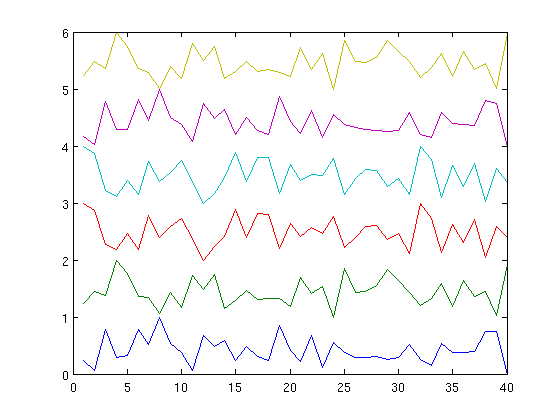
\includegraphics[width=\textwidth]{rep2.png}
\end{subfigure}

\begin{subfigure}[b]{0.3\textwidth}
	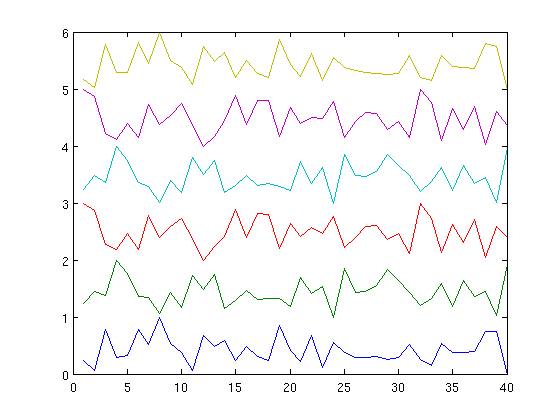
\includegraphics[width=\textwidth]{rep3.png}
\end{subfigure}

\caption{The bottom 3 lines are original signals from
\texttt{icaTest.mat}. The top 3 lines are reconstructed signals with
$\eta = 0.01$ and 1000000 iterations.}
\label{fig:rep}
\end{figure}

Frobenius Norm.

\section{Discussion}

\section{Conclusion}

\end{document}
